\setchapterimage[8.5cm]{tde}
\setchapterpreamble[u]{\margintoc}
\chapter{Neutrino Cosmology}
\labch{neutrino_cosmology}
\begin{fquote}[ Kurt Vonnegut][The Design of Experiments][1935]The universe is a big place, perhaps the biggest.
\end{fquote}

Often, the strictest limits on the contribution of a given source class comes not from direct likelihood analysis, but rather from much simpler cosmological arguments. IceCube measures a diffuse astrophysical neutrino flux, setting a limit on the cumulative contribution that can come from a given population. This information can be illustrated by a \emph{Kowalski Plot}, encompassing the product of a local rate and a mean neutrino luminosity per source. 

As part of this thesis, a software framework was developed to analytically calculate neutrino emission from cosmological populations. This is integrated into the \emph{\href{https://github.com/IceCubeOpenSource/flarestack}{Flarestack}} python package, written by the author \sidecite{flarestack}.

\section{Calculating a diffuse neutrino flux}

Populations of astrophysical transients are characterised by their \emph{local rate} (how often they occur in the local universe), and their source evolution (how does their rate change as a function of redshift). Rates are typically estimated from unbiased surveys, such as the ZTF Bright Transient Survey. Since many astrophysical transients outlined in Chapter \ref{ch:sources} are ultimately related to stages of stellar evolution, they tend to be strongly correlated to the \emph{Star Formation Rate} (SFR), the rate at which stars are formed at a given redshift.

The SFR can be directly inferred using multi-wavelength surveys of galaxies \sidecite{sfr_madau_14}, exploiting the characteristic spectral ratios to quantify stellar contributions in each galaxy. Alternatively, the SFR rate can be indirectly derived using observed rates of core-collapse supernovae identified in surveys \sidecite{sfr_strolger_15}. These two rates are illustrated in Figure N, and broadly agree. The SFR peaks at z$\approx$1 because of REASONS, and declines thereafter. It has a \emph{positive evolution}, i.e it increases with increasing redshift. 

An alternative driver of evolution is the rate of supermassive black holes (SMBHs), which are connected with many other sources such as blazars, radio galaxies and TDEs. In contrast to the SFR, massive SMBHs are thought to be formed through mergers of smaller SMBHs. The rate of massive SMBHs has a tendency to increase over time, so is larger in the local universe than at higher redshifts. In contrast to the SFR, the SMBH rate this has a \emph{negative source evolution}. Of particular relavance to this thesis is the rate of TDEs, which have been proposed theoretically to follow this negative SMBH rate, as illustrated in Figure N \sidecite{Sun:2015bda}. Caution must be taken for this rate, since TDEs are primarily detected in the local universe, so the high-z rates are broadly unconstrained observationally.

While the limits presented above constrain the contribution of those catalogues tested, we ultimately wish to constrain neutrino emission for the TDE population as a whole. If we \emph{assume that catalogue sources are representative of the broader population}, we can extrapolate from our per-source standard candle limits in Figure \ref{fig:cat_upper_limit} to the population flux. We seek to constrain the flux of two populations, namely jetted and non-jetted TDEs. For the latter case, we rely on the results of the golden TDE catalogue, since the extrapolation \emph{implicitly requires that the catalogues are not contaminated by misclassified objects}.

We must multiply the energy-per-source by the rate of TDEs as a function of redshift, yielding an energy-per-redshift-shell. We can then scale with the luminosity distance to derive the flux-per-shell at Earth. By numerically integrating the flux contributed by shells of increasing redshift up to a horizon of z=8, we thus calculate the cumulative flux expected for each population. This method thus accounts for TDEs that were not detected by other surveys, and were therefore not incorporated into our catalogue. 

There a number of subtleties to this method. The rate is given per unit time, but the impact of time dilation at higher redshifts suppresses the rate by a factor (1+z). Furthermore, in much the same way as for photons, neutrinos from distant shells will be "red-shifted" to lower energies. At Earth, for energy $E_{\textup{obs}}$, we will observe neutrinos that were emitted at $E_{\textup{em}} = (1+z) E_{\textup{obs}}$. Thus, for a power law of E$^{-\gamma}$, the flux at $E_{\textup{obs}}$ will be suppressed by a factor of $(1+z) ^{\gamma}$. Both effects are generally small for the sources in the catalogue, because it primarily probes the local universe, but must be accounted for when extrapolating.

To perform this calculation, we use per-source limits for the most recent IceCube global fit of the astrophysical neutrino flux, with a best-fit spectrum of $E^{-2.50}$. For non-jetted TDEs, we assume a central local rate of $8 \times 10^{-7}$ Mpc$^{-3}$ year$^{-1}$ \sidecite{2018ApJ...852...72V}, a source evolution derived by \cite{Sun:2015bda}, and constrain the contribution of TDEs to be less than 26\% of the total. For jetted TDEs, under the assumption that they follow the same underlying source evolution as non-jetted TDEs with a central rate of $3 \times 10^{-11}$ Mpc$^{-3}$ year$^{-1}$ \sidecite{Sun:2015bda}, we find that they must contribute less than 1\% of the total.  These constraints are illustrated in Figure \ref{fig:DiffuseFlux}.

As the contribution from a population is directly proportional to the local population rate, the shaded bands indicate the uncertainty in our limits arising from rate estimates. For TDEs, these rates are the dominant source of uncertainty in neutrino flux. It will require systematic evaluation of observed TDE rates to enable more precise limits on neutrino emission. Any refined rate estimate can be used to linearly rescale these limits. Propagating through the current local rate uncertainty, we constrain non-jetted TDEs to be less than 13-39\%, and jetted TDEs to be less than 0.n-1.n\% of the total. With a more precise future measurement of the local TDE rate, these values can be linearly rescaled to provide more accurate limits.

Such limits also critically depend on the source evolution of TDEs as a function of redshift, but this is essentially unconstrained observationally because TDEs detections are overwhelmingly confined to the local universe (z $\lesssim$ 0.3). Estimates are made primarily based on theoretical predictions derived from the rate of SuperMassive Black Holes (SMBHs)?? \cite{Sun:2015bda}. If we instead consider a source evolution similar to the Star Formation Rate (SFR), as derived by CLASH-CANDELs, we would find limits of x and y \% respectively. For such a scenario, the contribution of unresolved TDEs is so large that the measured flux itself provides a stricter constraint than the catalogue test?

\section{Comparing Rate Evolutions}

\begin{marginfigure}
	\centering 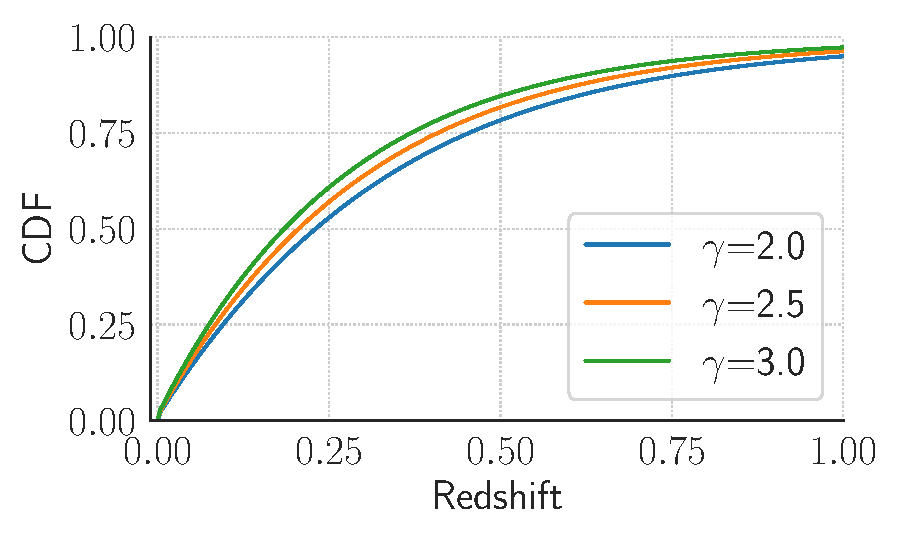
\includegraphics{nu_cosmology/flux_gamma}
	\caption{Cumulative flux as a function of spectral index.}
	\label{fig:CDF_gamma}
\end{marginfigure}


\begin{marginfigure}
	\centering 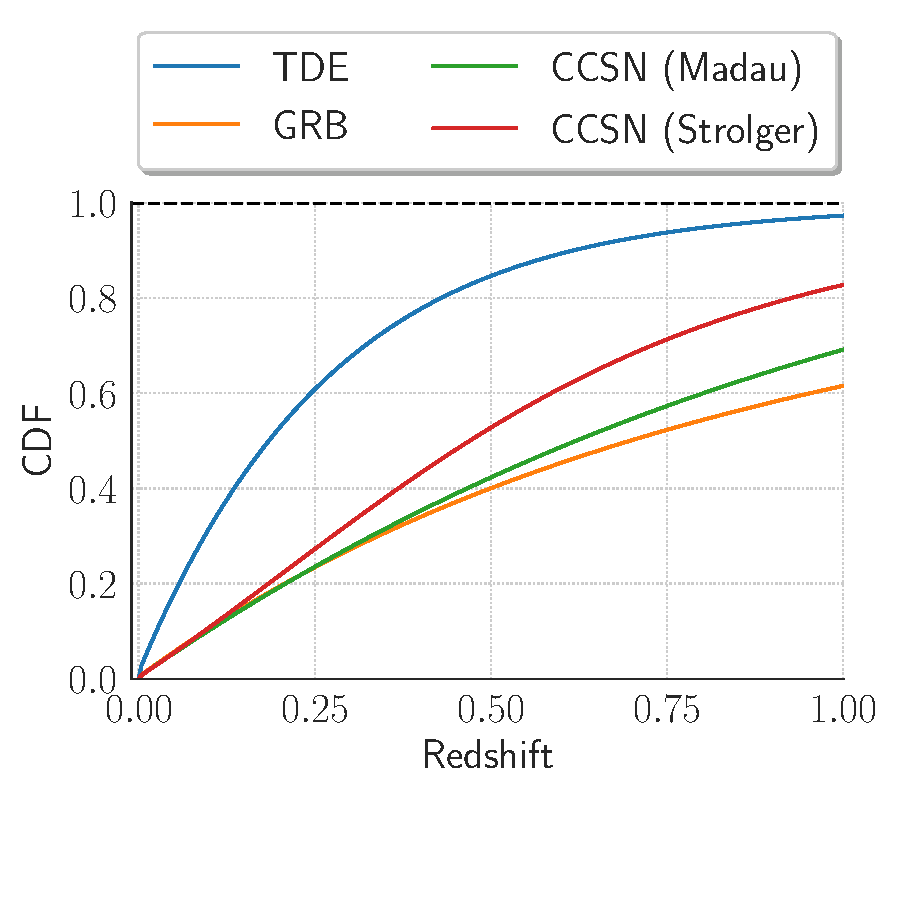
\includegraphics{nu_cosmology/diffuse_flux_rates}
	\caption{Cumulative flux as a function of source evolution.}
	\label{fig:CDF_rate}
\end{marginfigure}

\begin{marginfigure}
	\centering 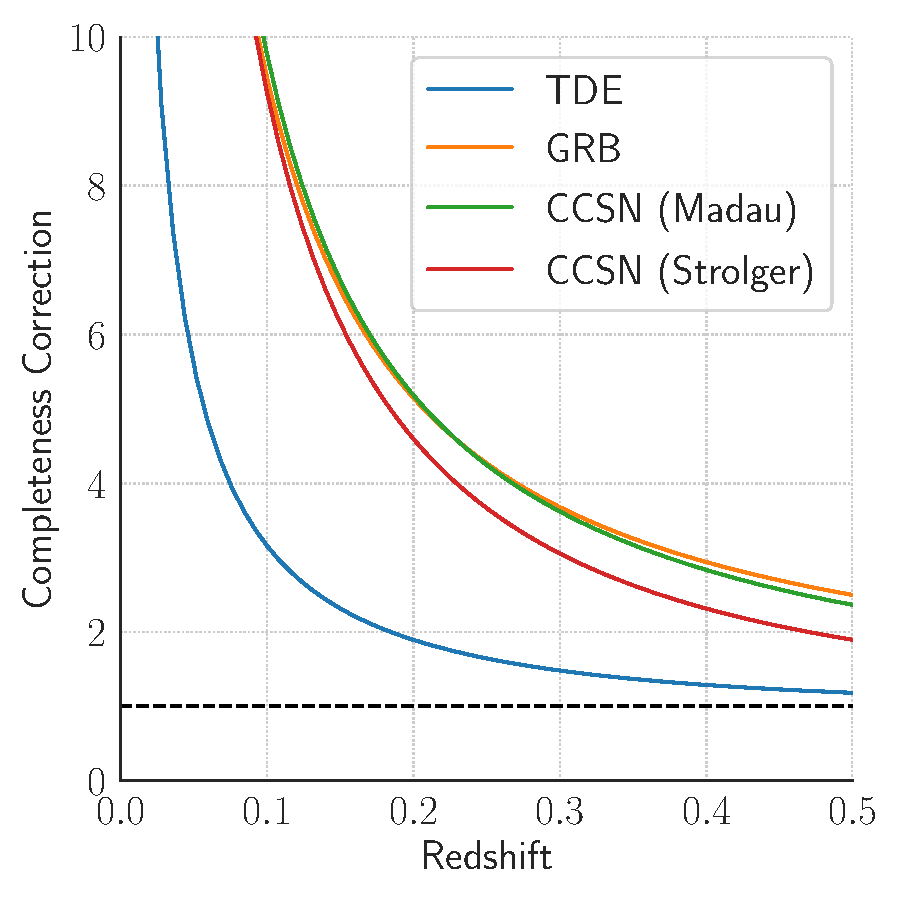
\includegraphics{nu_cosmology/diffuse_flux_completeness}
	\caption{Completeness correction factor as a function of source evolution.}
	\label{fig:completeness}
\end{marginfigure}

Figure \ref{fig:completeness} illustrates the completeness correction factor as a function of redshift. For a sample complete up to a redshift of z, multiplying the sample flux by the correction factor will yield the total population flux. An alternative interpretation is that this factor is the number of population neutrinos that would need to be followed up before a counterpart was identified, assuming that the follow-up instruments were sensitive up to redshift z. This Figure illustrates most starkly the challenge of optical follow-up of neutrinos, and the relative sensitivity to different source evolutions. For a negative rate, the cumulative neutrino flux of TDEs will be overwhelmingly dominated by nearby sources, while transients that evolve with the Star Formation Rate (e.g CCSNe) have a much larger contribution from more distant sources.

To give a specific example, ZTF is approximately complete in identifying TDEs up to a redshift of 0.15. Per Figure \ref{fig:CDF_rate}, this volume will contain sources responsible for roughly 35\% of the population flux, and from Figure \ref{fig:completeness}, we see that we would expect to find roughly 1/3 of counterparts to TDE neutrinos. In contrast, CCSNe tend to be dimmer, and so we would be complete primarily up to a redshift of z=0.1?. Even neglecting this effect, with SFR-evolution only 10\% of neutrinos will be produced in the volume z<0.15.

To approximately quantify the impact of this effect, we can consider the general power of tests probing this region. The signal, $\mathcal{S}$ is proportional to the fraction of flux belonging to resolvable sources, while the background rate, $\mathcal{B}$, is proportional to the number of sources within this volume.

We consider a neutrino with typical properties for those issued as IceCube realtime alerts. We assume it has a \emph{signalness} of 50\%, i.e that it has a 50\% probability to be of astrophysical origin rather than from atmospheric backgrounds. Such alerts are typically reported with a median angular error of $\sim$1 degree. Any source class will then have a cumulative expectation of 0.5 $\times f_{\textup{tot}}$, where $f_{\textup{tot}}$ is the fraction of the total diffuse astrophysical neutrino flux contributed by that source class. 
		
We consider a number of source classes, listed in Table N. We calculate their expected background rate by considering their sky rate, given as a product of their local rate, integrated to a typical telescope horizon, and multiplied by a typical telescope detection efficiency. For each source, we also multiply the appropriate search window for neutrino emission, yielding a final background density for any point on the sky. Multiplying this by the neutrino localisation area gives us the ultimate background rate per follow-up. We also consider the expected signal per search, given as the neutrino population expectation multiplied by the fraction of flux which is produced by sources accessible to telescopes.  These are illustrated in Figure \ref{fig:nsig_nbkg} for a variety of source classes.

\begin{figure}[!ht]
	\centering 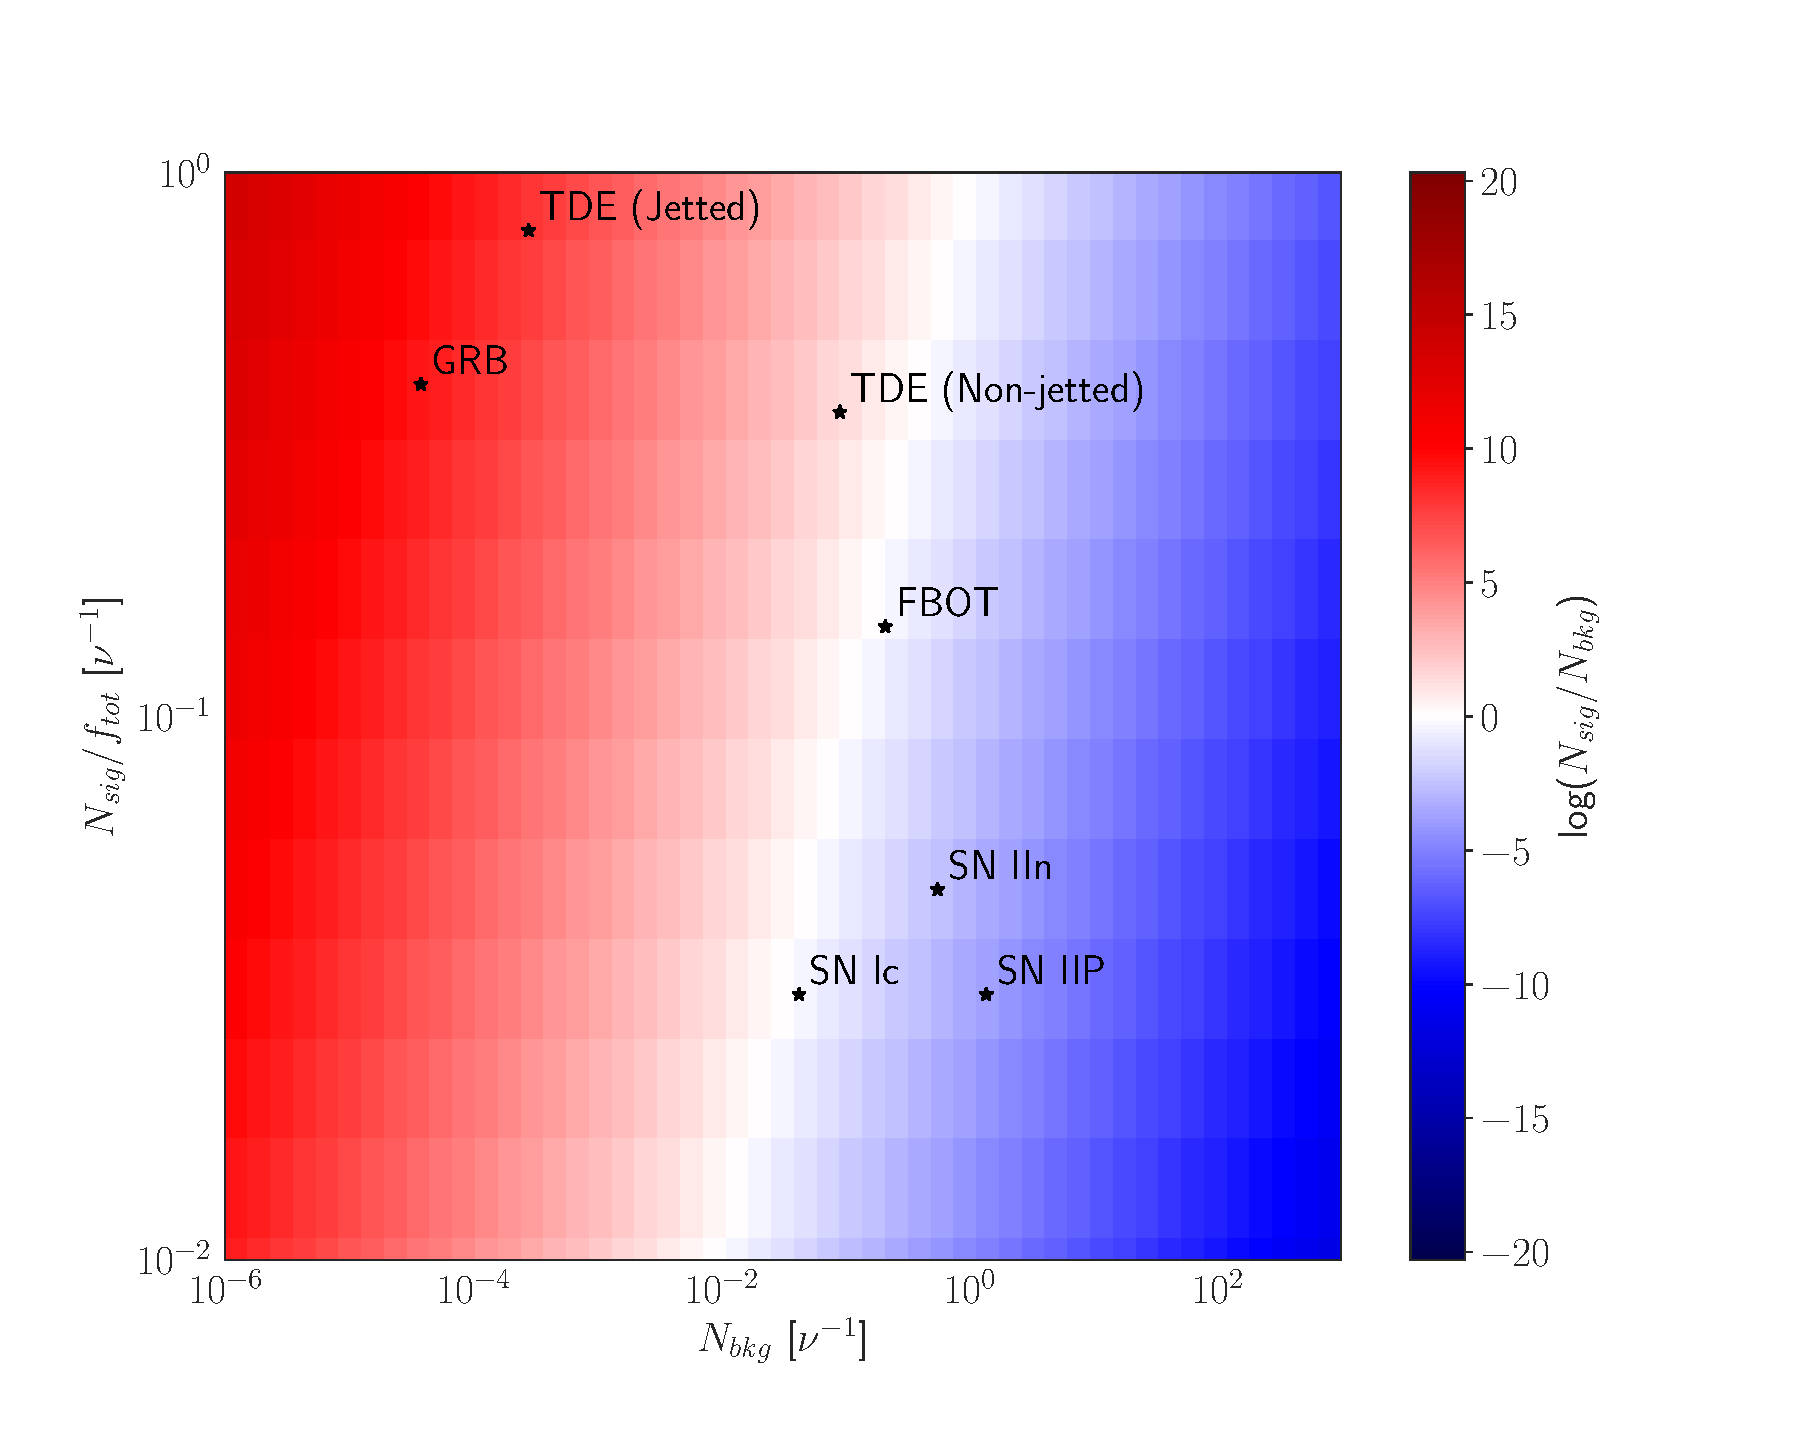
\includegraphics{nu_cosmology/nsig_nbkg}
	\caption{Nsig vs Nbkg}
	\label{fig:nsig_nbkg}
\end{figure}

The intrinsic signal-to-noise of different source classes can be seen, with the white band indicating the transition from the red signal-dominated regions to the blue background-dominated regions. In general, the probability of observing a coincidence increases from lower left to upper right, while the significance of any coincidence increases from lower right to upper left. For sources with $N_{\textup{bkg}} \lesssim 0.1$, where the probability of multiple background events is negligible, the x axis represents the p-value for a coincidence. By analogy, the y axis represents the probability of observing a coincidence.

Though Figure \ref{fig:nsig_nbkg} contains no analysis of IceCube data, it is particularly notable that the position of sources correspond very directly to the relative constraints that have been placed on those classes by IceCube. Neutrino-specific properties of signalness and localisation will linearly scale all points in the x or y direction respectively, but the relative positions of sources remains unchanged. Those sources near the top of the Figure are those with the strictest existing limits, often at percent-level, while those nearer the lower/lower-right portion are only weakly constrained or could still produce the entire diffuse flux. 

One particularly noteworthy class is FRBs, which are particularly favourable owing to their extremely stringent temporal localisation. Indeed, were telescopes fully efficient at detecting these across the sky, the limits on this class would be perhaps the most stringent of all. However, at the time of the most recent IceCube analysis, 21 FRBs were tested against an estimated rate of 3000 per sky per day, a sample for which no constraint could be placed on the FRB population \sidecite{icrc_frb}. It is precisely because the detection efficiency of FRBs is so low that a tiny fraction of signal is detectable. The expected signal to background ratio for FRBs is very high, and this statement is independent of detection efficiency, so any FRB-neutrino coincidence would be very strong evidence for a physical association. However, because the probability that an FRB counterpart would be detected at all is so low at present, no coincidence is likely to be found. The corresponding FRB (IC) position is illustrated, with an implied detection efficiency of N\%. 

The plot illustrates how well the full unbinned likelihood analysis method used by IceCube for neutrino astronomy can in fact be approximated by a poisson counting experiment.

\begin{figure}[!ht]
	\centering 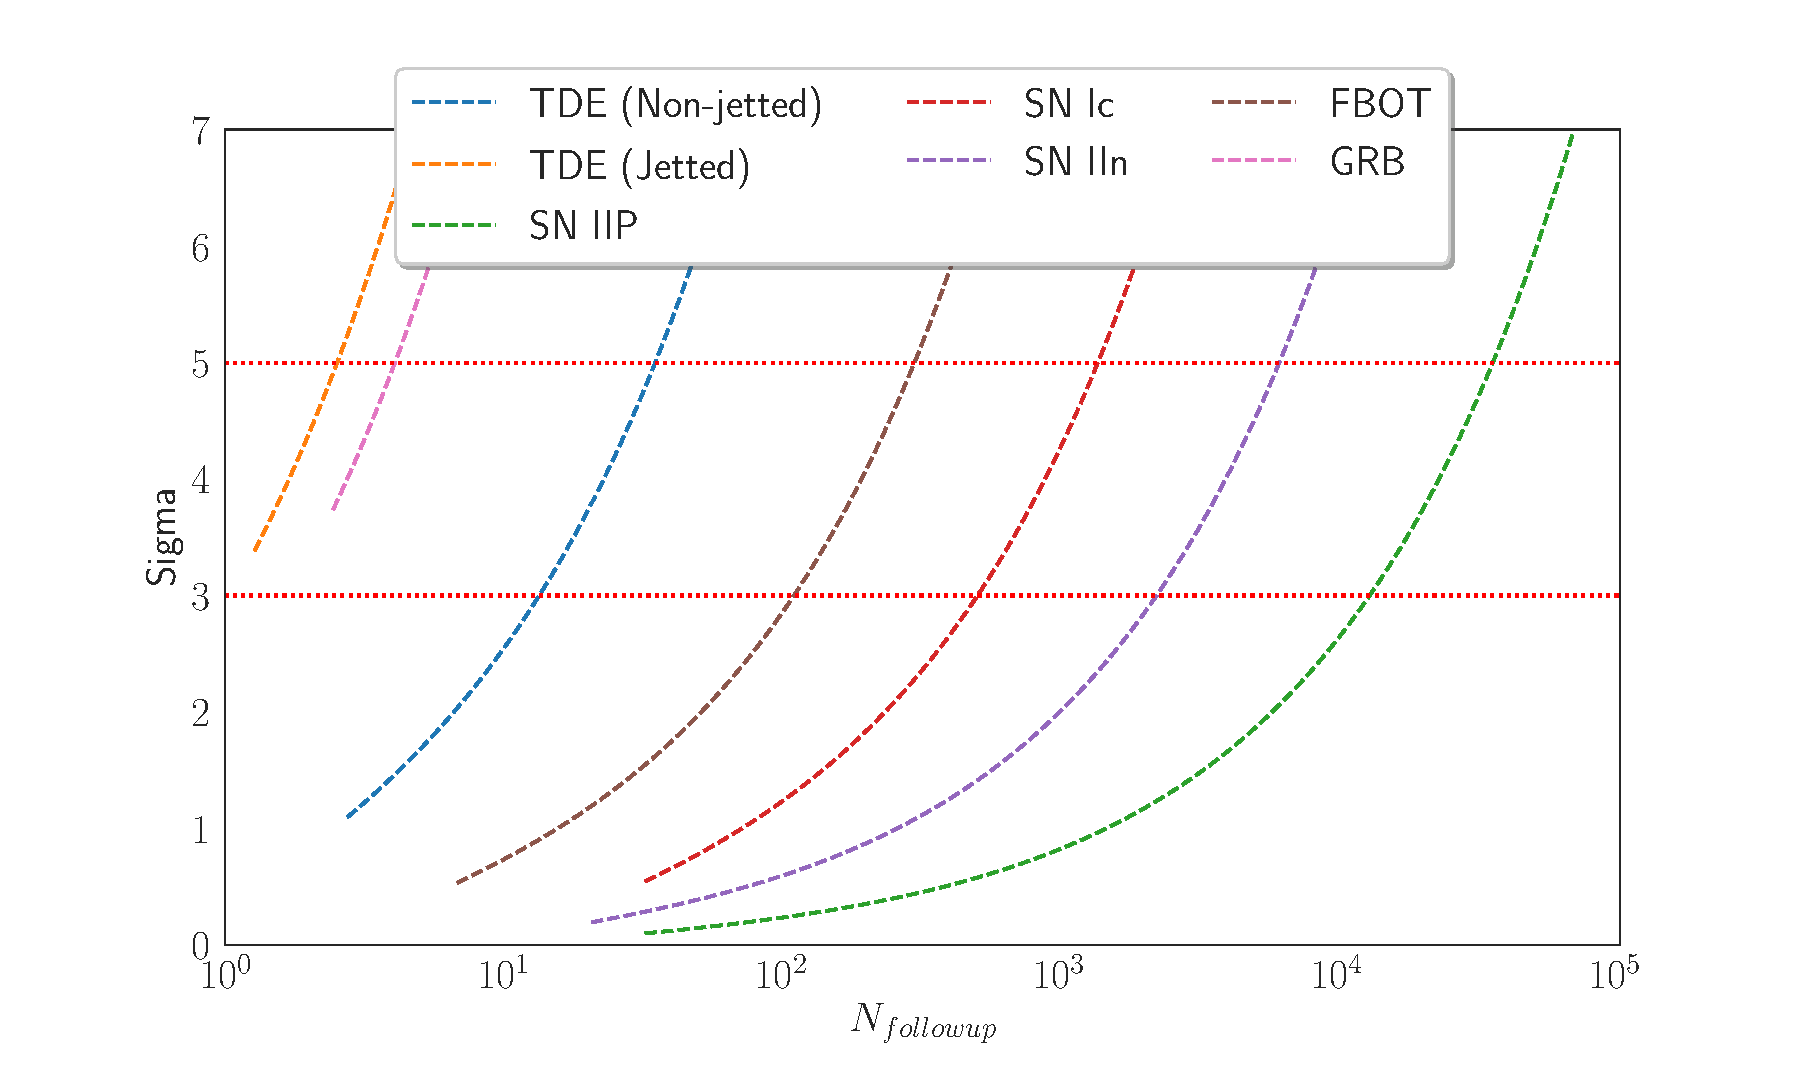
\includegraphics{nu_cosmology/p_value_nfollowup}
	\caption{Statistical significance of excess coincidence as a function of number of follow-up}
	\label{fig:p_value}
\end{figure}
